\documentclass[portrait,final,a0paper,fontscale=0.277]{baposter}

\usepackage{calc}
\usepackage{graphicx}
\usepackage{amsmath}
\usepackage{amssymb}
\usepackage{relsize}
\usepackage{multirow}
\usepackage{rotating}
\usepackage{bm}
\usepackage{url}

\usepackage{graphicx}
\usepackage{multicol}

%\usepackage{times}
%\usepackage{helvet}
%\usepackage{bookman}
\usepackage{palatino}

\newcommand{\captionfont}{\footnotesize}

\graphicspath{{images/}{../images/}}
\usetikzlibrary{calc}

\newcommand{\SET}[1]  {\ensuremath{\mathcal{#1}}}
\newcommand{\MAT}[1]  {\ensuremath{\boldsymbol{#1}}}
\newcommand{\VEC}[1]  {\ensuremath{\boldsymbol{#1}}}
\newcommand{\Video}{\SET{V}}
\newcommand{\video}{\VEC{f}}
\newcommand{\track}{x}
\newcommand{\Track}{\SET T}
\newcommand{\LMs}{\SET L}
\newcommand{\lm}{l}
\newcommand{\PosE}{\SET P}
\newcommand{\posE}{\VEC p}
\newcommand{\negE}{\VEC n}
\newcommand{\NegE}{\SET N}
\newcommand{\Occluded}{\SET O}
\newcommand{\occluded}{o}

%%%%%%%%%%%%%%%%%%%%%%%%%%%%%%%%%%%%%%%%%%%%%%%%%%%%%%%%%%%%%%%%%%%%%%%%%%%%%%%%
%%%% Some math symbols used in the text
%%%%%%%%%%%%%%%%%%%%%%%%%%%%%%%%%%%%%%%%%%%%%%%%%%%%%%%%%%%%%%%%%%%%%%%%%%%%%%%%

%%%%%%%%%%%%%%%%%%%%%%%%%%%%%%%%%%%%%%%%%%%%%%%%%%%%%%%%%%%%%%%%%%%%%%%%%%%%%%%%
% Multicol Settings
%%%%%%%%%%%%%%%%%%%%%%%%%%%%%%%%%%%%%%%%%%%%%%%%%%%%%%%%%%%%%%%%%%%%%%%%%%%%%%%%
\setlength{\columnsep}{1.5em}
\setlength{\columnseprule}{0mm}

%%%%%%%%%%%%%%%%%%%%%%%%%%%%%%%%%%%%%%%%%%%%%%%%%%%%%%%%%%%%%%%%%%%%%%%%%%%%%%%%
% Save space in lists. Use this after the opening of the list
%%%%%%%%%%%%%%%%%%%%%%%%%%%%%%%%%%%%%%%%%%%%%%%%%%%%%%%%%%%%%%%%%%%%%%%%%%%%%%%%
\newcommand{\compresslist}{%
\setlength{\itemsep}{1pt}%
\setlength{\parskip}{0pt}%
\setlength{\parsep}{0pt}%
}

%%%%%%%%%%%%%%%%%%%%%%%%%%%%%%%%%%%%%%%%%%%%%%%%%%%%%%%%%%%%%%%%%%%%%%%%%%%%%%
%%% Begin of Document
%%%%%%%%%%%%%%%%%%%%%%%%%%%%%%%%%%%%%%%%%%%%%%%%%%%%%%%%%%%%%%%%%%%%%%%%%%%%%%

\begin{document}

%%%%%%%%%%%%%%%%%%%%%%%%%%%%%%%%%%%%%%%%%%%%%%%%%%%%%%%%%%%%%%%%%%%%%%%%%%%%%%
%%% Here starts the poster
%%%---------------------------------------------------------------------------
%%% Format it to your taste with the options
%%%%%%%%%%%%%%%%%%%%%%%%%%%%%%%%%%%%%%%%%%%%%%%%%%%%%%%%%%%%%%%%%%%%%%%%%%%%%%
% Define some colors

%\definecolor{lightblue}{cmyk}{0.83,0.24,0,0.12}
\definecolor{lightblue}{rgb}{0.145,0.6666,1}

% Draw a video
\newlength{\FSZ}
\newcommand{\drawvideo}[3]{% [0 0.25 0.5 0.75 1 1.25 1.5]
   \noindent\pgfmathsetlength{\FSZ}{\linewidth/#2}
   \begin{tikzpicture}[outer sep=0pt,inner sep=0pt,x=\FSZ,y=\FSZ]
   \draw[color=lightblue!50!black] (0,0) node[outer sep=0pt,inner sep=0pt,text width=\linewidth,minimum height=0] (video) {\noindent#3};
   \path [fill=lightblue!50!black,line width=0pt] 
     (video.north west) rectangle ([yshift=\FSZ] video.north east) 
    \foreach \x in {1,2,...,#2} {
      {[rounded corners=0.6] ($(video.north west)+(-0.7,0.8)+(\x,0)$) rectangle +(0.4,-0.6)}
    }
;
   \path [fill=lightblue!50!black,line width=0pt] 
     ([yshift=-1\FSZ] video.south west) rectangle (video.south east) 
    \foreach \x in {1,2,...,#2} {
      {[rounded corners=0.6] ($(video.south west)+(-0.7,-0.2)+(\x,0)$) rectangle +(0.4,-0.6)}
    }
;
   \foreach \x in {1,...,#1} {
     \draw[color=lightblue!50!black] ([xshift=\x\linewidth/#1] video.north west) -- ([xshift=\x\linewidth/#1] video.south west);
   }
   \foreach \x in {0,#1} {
     \draw[color=lightblue!50!black] ([xshift=\x\linewidth/#1,yshift=1\FSZ] video.north west) -- ([xshift=\x\linewidth/#1,yshift=-1\FSZ] video.south west);
   }
   \end{tikzpicture}
}

\hyphenation{resolution occlusions}
%%
\begin{poster}%
  % Poster Options
  {
  % Show grid to help with alignment
  grid=false,
  % Column spacing
  colspacing=1em,
  % Color style
  bgColorOne=white,
  bgColorTwo=white,
  borderColor=lightblue,
  headerColorOne=black,
  headerColorTwo=lightblue,
  headerFontColor=white,
  boxColorOne=white,
  boxColorTwo=lightblue,
  % Format of textbox
  textborder=roundedleft,
  % Format of text header
  eyecatcher=true,
  headerborder=closed,
  headerheight=0.1\textheight,
%  textfont=\sc, An example of changing the text font
  headershape=roundedright,
  headershade=shadelr,
  headerfont=\Large\bf\textsc, %Sans Serif
  textfont={\setlength{\parindent}{1.5em}},
  boxshade=plain,
%  background=shade-tb,
  background=plain,
  linewidth=2pt
  }
  % Eye Catcher
  {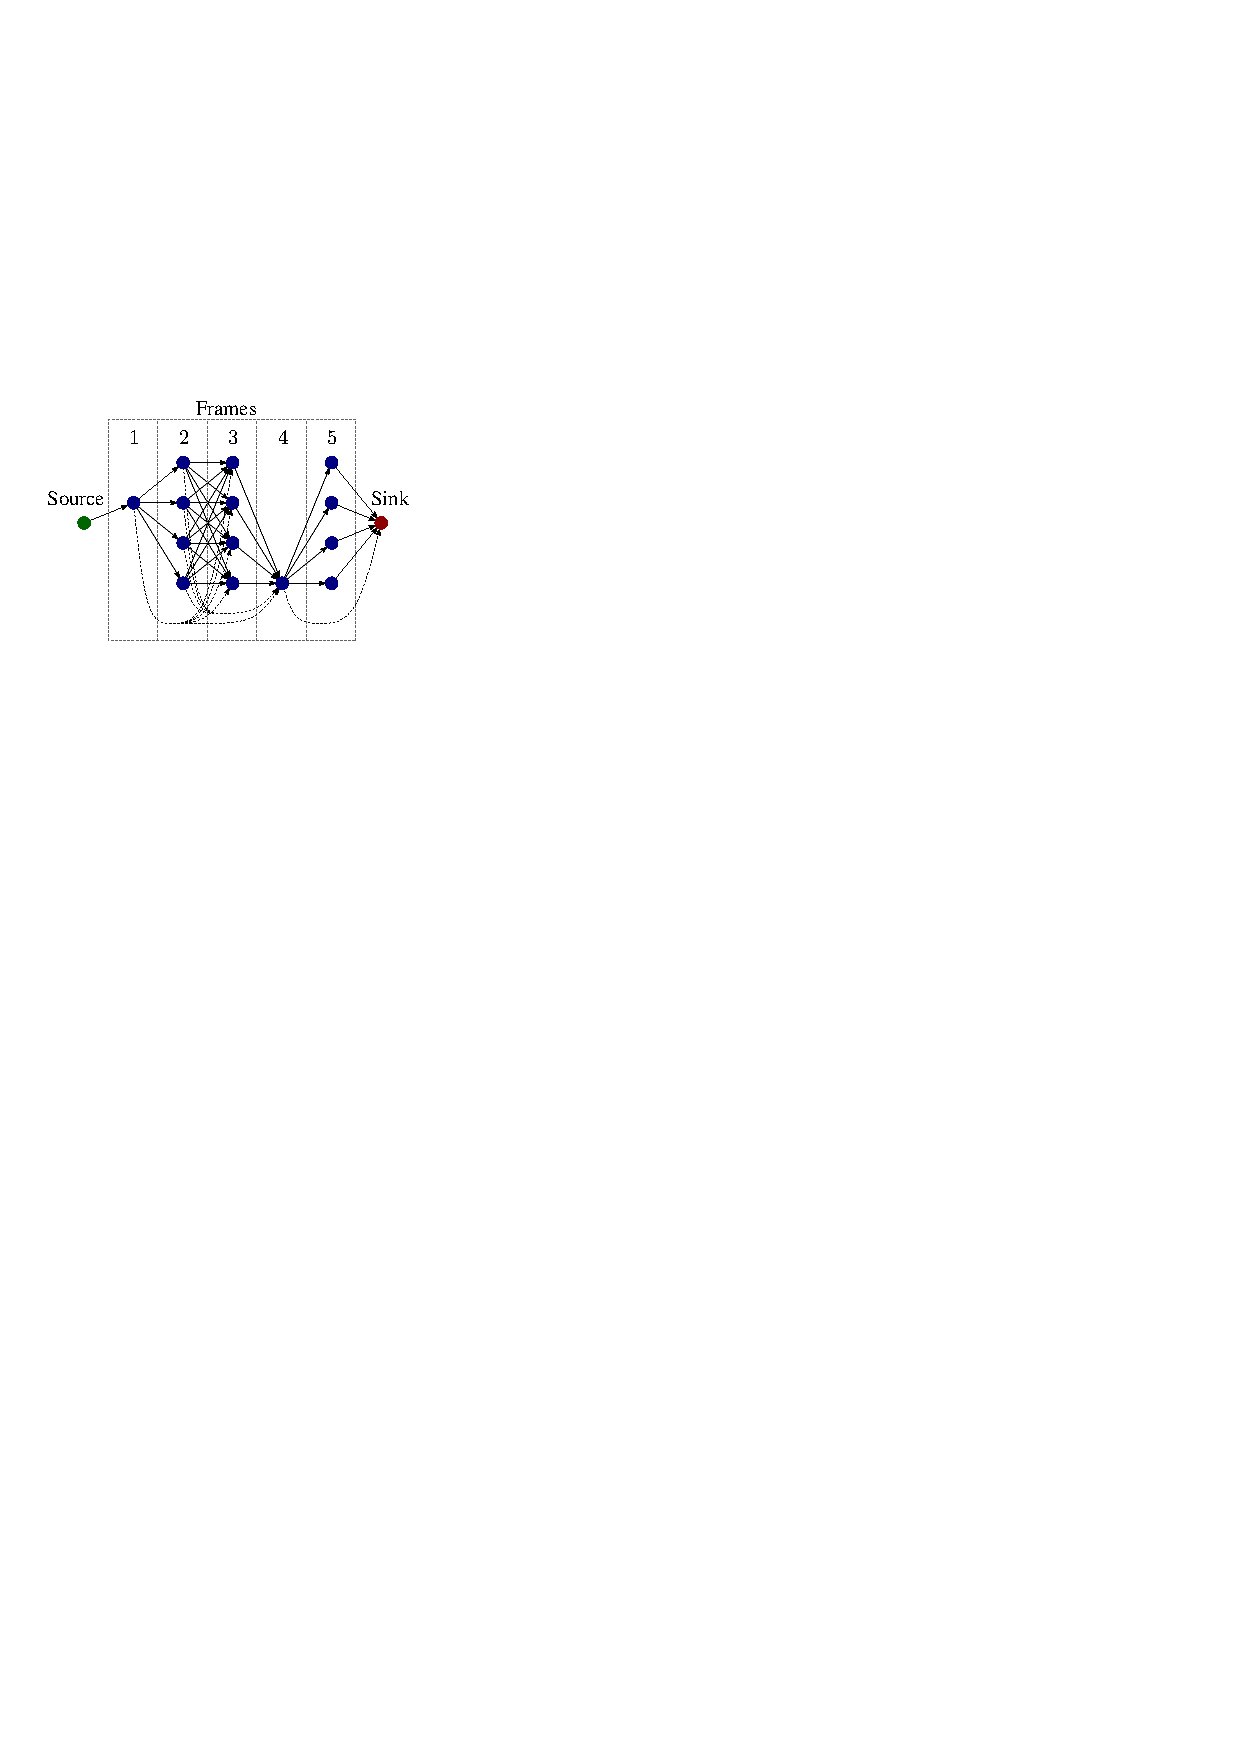
\includegraphics[height=5em]{images/graph_occluded.pdf}} 
  % Title
  {\bf\textsc{GraphTrack: Fast and Globally Optimal Tracking in Videos}\vspace{0.5em}}
  % Authors
  {\textsc{\{ Brian.Amberg and Thomas.Vetter \}@unibas.ch}}
  % University logo
  {% The makebox allows the title to flow into the logo, this is a hack because of the L shaped logo.
    
\includegraphics[height=9.0em]{images/logo}
  }

%%%%%%%%%%%%%%%%%%%%%%%%%%%%%%%%%%%%%%%%%%%%%%%%%%%%%%%%%%%%%%%%%%%%%%%%%%%%%%
%%% Now define the boxes that make up the poster
%%%---------------------------------------------------------------------------
%%% Each box has a name and can be placed absolutely or relatively.
%%% The only inconvenience is that you can only specify a relative position 
%%% towards an already declared box. So if you have a box attached to the 
%%% bottom, one to the top and a third one which should be in between, you 
%%% have to specify the top and bottom boxes before you specify the middle 
%%% box.
%%%%%%%%%%%%%%%%%%%%%%%%%%%%%%%%%%%%%%%%%%%%%%%%%%%%%%%%%%%%%%%%%%%%%%%%%%%%%%
    %
    % A coloured circle useful as a bullet with an adjustably strong filling
    \newcommand{\colouredcircle}{%
      \tikz{\useasboundingbox (-0.2em,-0.32em) rectangle(0.2em,0.32em); \draw[draw=black,fill=lightblue,line width=0.03em] (0,0) circle(0.18em);}}

%%%%%%%%%%%%%%%%%%%%%%%%%%%%%%%%%%%%%%%%%%%%%%%%%%%%%%%%%%%%%%%%%%%%%%%%%%%%%%
  \headerbox{Problem}{name=problem,column=0,row=0}{
%%%%%%%%%%%%%%%%%%%%%%%%%%%%%%%%%%%%%%%%%%%%%%%%%%%%%%%%%%%%%%%%%%%%%%%%%%%%%%
   Tracks of features through scenes are needed for data analysis, as well as
   for movie special effects. Tracks are found in an interactive process. The
     artist marks a position, and the computer proposes a track which is then
     further refined by the artist.

   This is a difficult problem due to three aspects. 
   \begin{enumerate}\compresslist
      \item Appearance changes due to lighting and pose
      \item Occlusions
      \item Speed: Interactive editing requires faster than framerate calculation
   \end{enumerate}
   \vspace{0.3em}
 }

%%%%%%%%%%%%%%%%%%%%%%%%%%%%%%%%%%%%%%%%%%%%%%%%%%%%%%%%%%%%%%%%%%%%%%%%%%%%%%
  \headerbox{Contributions}{name=contribution,column=0,below=problem}{
%%%%%%%%%%%%%%%%%%%%%%%%%%%%%%%%%%%%%%%%%%%%%%%%%%%%%%%%%%%%%%%%%%%%%%%%%%%%%%
   We formulated tracking as path search in a large graph, and solve it
   efficiently with a modificiation of Dijkstra's algorithm.  

   The method is based on \cite{awf:tracking}. Our main contributions are
   \begin{enumerate}\compresslist
   \item Efficient incorporation of a background appearance model
   \item Formulation as a shortest path problem
   \item (Correct) handling of occlusions
   \item High-Efficiency implementation with up to 150 fps for a high
   resolution video
   \end{enumerate}
   \vspace{0.3em}
  }

%%%%%%%%%%%%%%%%%%%%%%%%%%%%%%%%%%%%%%%%%%%%%%%%%%%%%%%%%%%%%%%%%%%%%%%%%%%%%%
\headerbox{Results}{name=results,column=1,span=2,row=0}{
  %%%%%%%%%%%%%%%%%%%%%%%%%%%%%%%%%%%%%%%%%%%%%%%%%%%%%%%%%%%%%%%%%%%%%%%%%%%%%%
    \drawvideo{5}{40}{%
      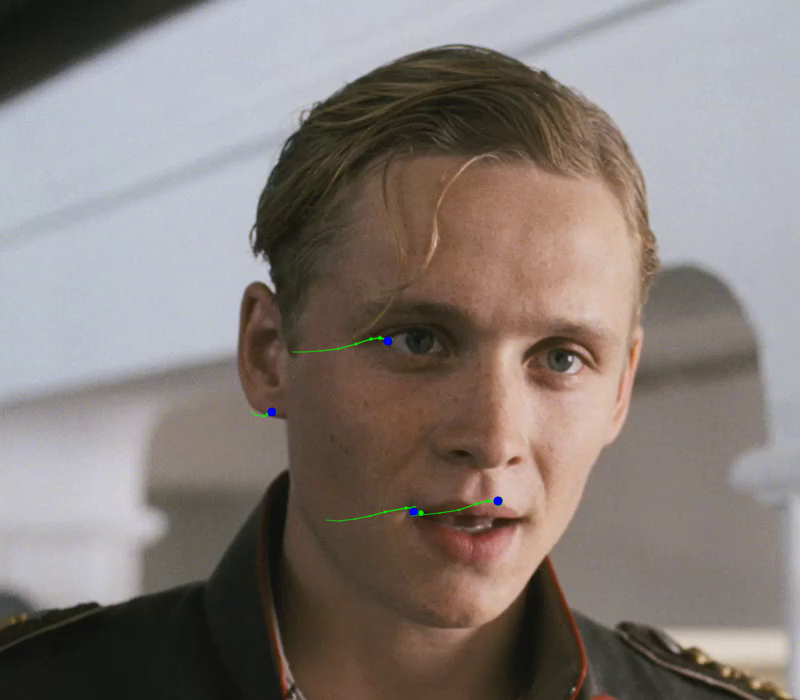
\includegraphics[width=0.2\linewidth]{red-4-sec_000_rastered}%
        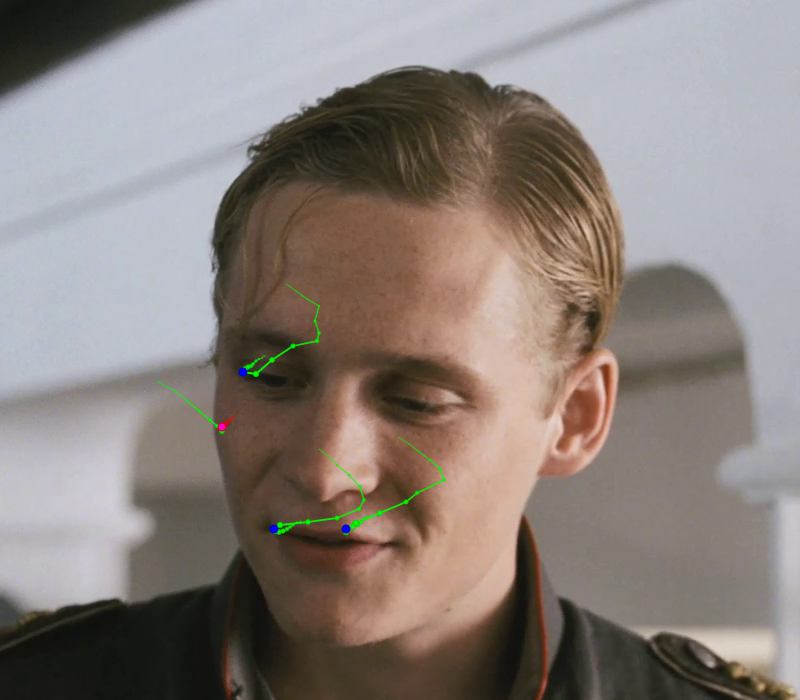
\includegraphics[width=0.2\linewidth]{red-4-sec_024_rastered}%
        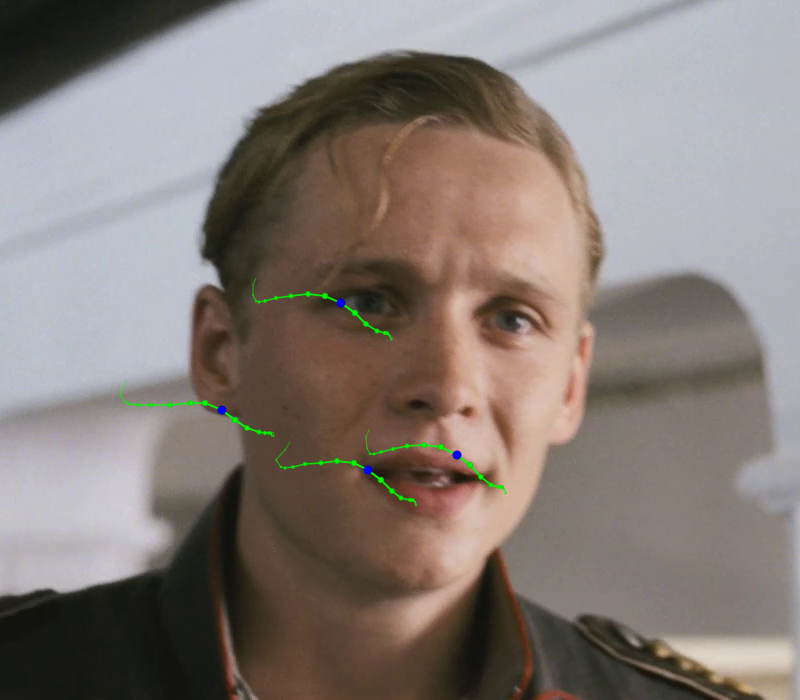
\includegraphics[width=0.2\linewidth]{red-4-sec_048_rastered}%
        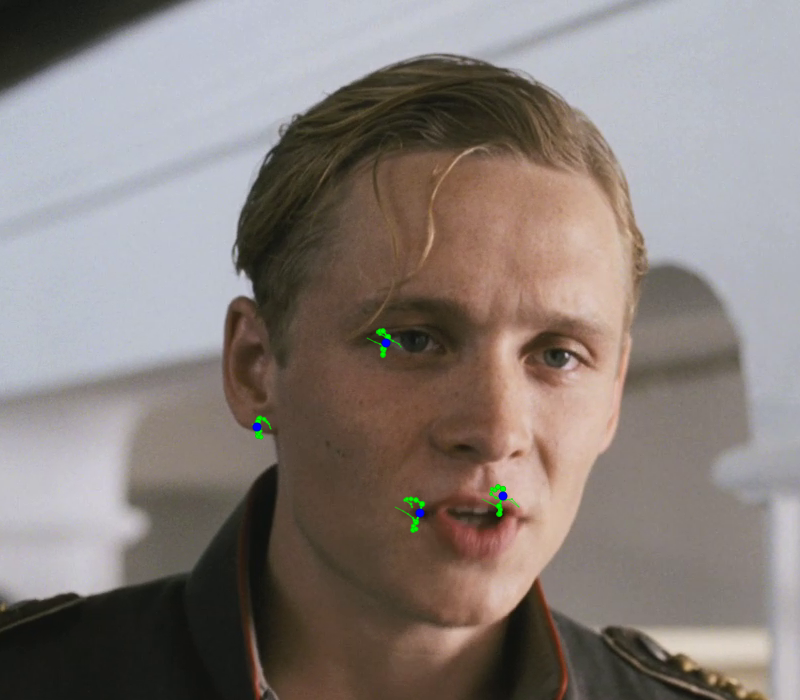
\includegraphics[width=0.2\linewidth]{red-4-sec_072_rastered}%
        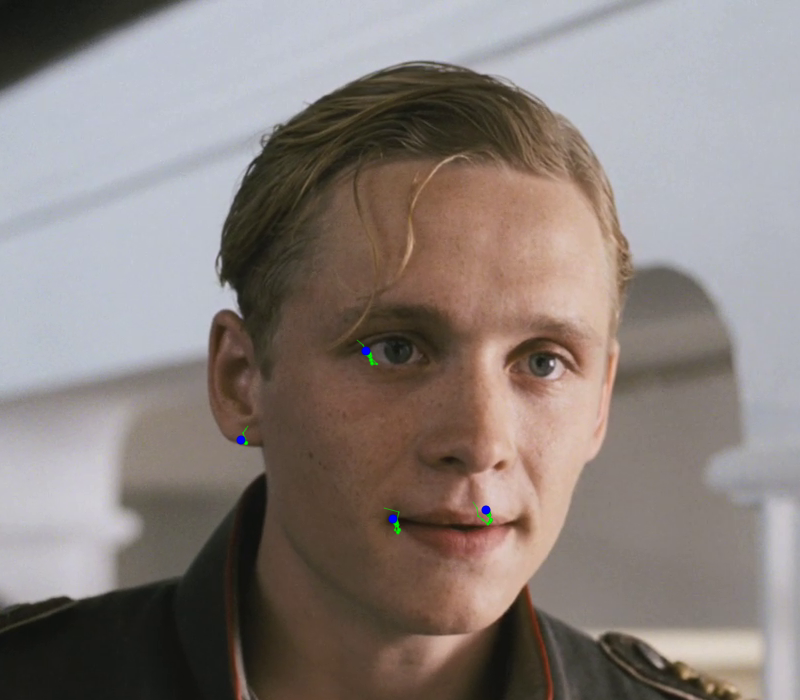
\includegraphics[width=0.2\linewidth]{red-4-sec_095_rastered}%
    }
  \begin{tabular*}{\linewidth}{*{5}{@{}p{0.2\linewidth}@{}}}
    {\hfill{}Frame 0\hfill{}} & {\hfill{}24\hfill{}} &  {\hfill{}48\hfill{}} &  {\hfill{}72\hfill{}} & {\hfill{}95\hfill{}}
  \end{tabular*}
  \\[1em]
      \drawvideo{5}{40}{%
        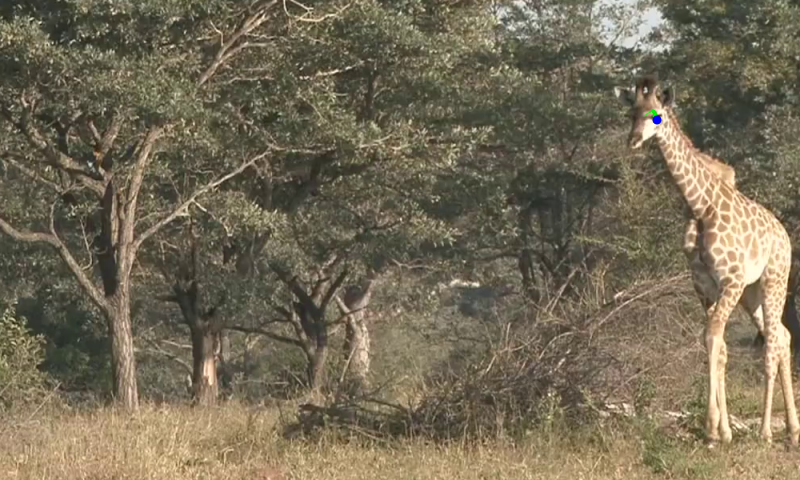
\includegraphics[width=0.2\linewidth]{giraffe-run-000-rastered}%
          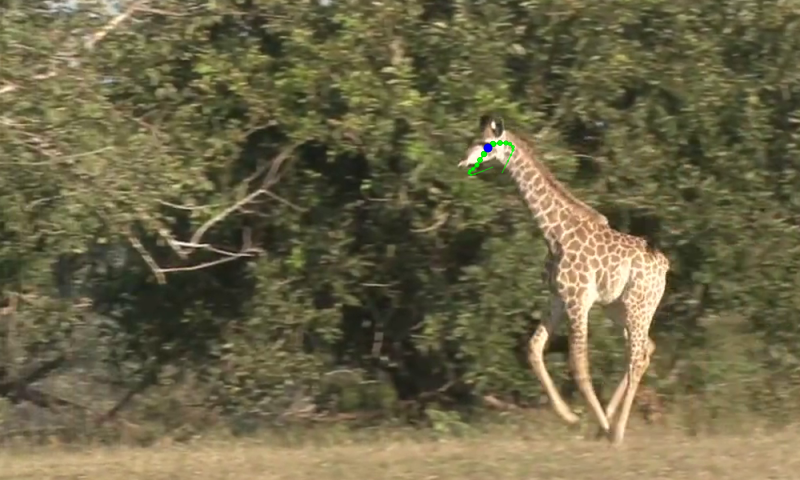
\includegraphics[width=0.2\linewidth]{giraffe-run-100-rastered}%
          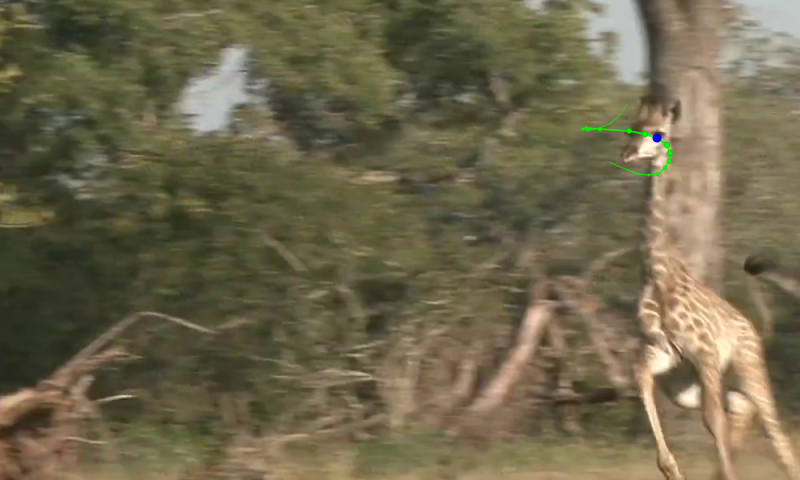
\includegraphics[width=0.2\linewidth]{giraffe-run-200-rastered}%
          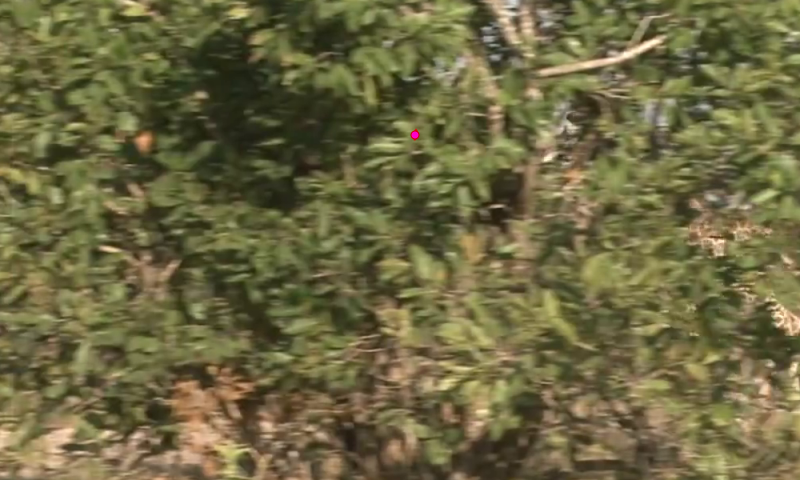
\includegraphics[width=0.2\linewidth]{giraffe-run-300-rastered}%
          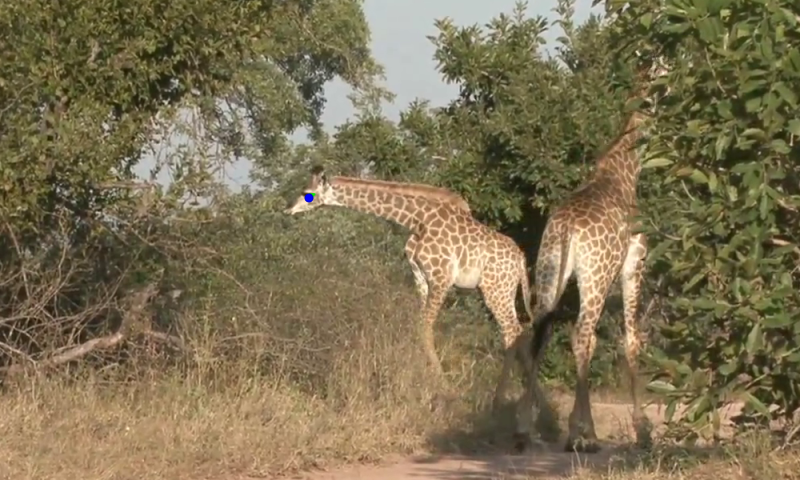
\includegraphics[width=0.2\linewidth]{giraffe-run-458-rastered}%
      }
  \begin{tabular*}{\linewidth}{*{5}{@{}p{0.2\linewidth}@{}}}
    {\hfill{}Frame 0\hfill{}}  &
    {\hfill{}100\hfill{}} &
    {\hfill{}200\hfill{}} &
    {\hfill{}300\hfill{}} &
    {\hfill{}458\hfill{}} 
  \end{tabular*}
      \begin{multicols}{2}
    Between one and three user clicks were needed to achieve accurate tracking for
      the head sequence. Note the correct handling of the occluded ear, which
      required only a single click. 

      The eye of the running giraffe required eight user interactions, of which three
      marked occlusions. 
      \end{multicols}
      \vspace{-0.6em}
}
%%%%%%%%%%%%%%%%%%%%%%%%%%%%%%%%%%%%%%%%%%%%%%%%%%%%%%%%%%%%%%%%%%%%%%%%%%%%%%
  \headerbox{References}{name=references,column=0,above=bottom}{
%%%%%%%%%%%%%%%%%%%%%%%%%%%%%%%%%%%%%%%%%%%%%%%%%%%%%%%%%%%%%%%%%%%%%%%%%%%%%%
    \smaller
    \bibliographystyle{ieee}
    \renewcommand{\section}[2]{\vskip 0.05em}
      \begin{thebibliography}{1}\itemsep=-0.01em
      \setlength{\baselineskip}{0.4em}
      \bibitem{amberg11:graphtrack}
        B.~Amberg, T. Vetter.
        \newblock {GraphTrack}: {F}ast and {G}lobally {O}ptimal {T}racking in {V}ideos
        \newblock In {\em CVPR '11}
      \bibitem{awf:tracking}
        A.~Buchanan and A.~Fitzgibbon.
        \newblock {I}nteractive {F}eature {T}racking using {K-D} {T}rees and {D}ynamic {P}rogramming.
        \newblock In {\em CVPR '06}
      \end{thebibliography}
   \vspace{0.3em}
  }
%%%%%%%%%%%%%%%%%%%%%%%%%%%%%%%%%%%%%%%%%%%%%%%%%%%%%%%%%%%%%%%%%%%%%%%%%%%%%%
  \headerbox{Background Model}{name=background model,column=1,below=results}{
%%%%%%%%%%%%%%%%%%%%%%%%%%%%%%%%%%%%%%%%%%%%%%%%%%%%%%%%%%%%%%%%%%%%%%%%%%%%%%
\noindent\begin{tabular}{@{\hspace{0.0em}}c@{\hspace{1.5em}}c@{\hspace{0.0em}}}
With & Without\\
background model & background model\\
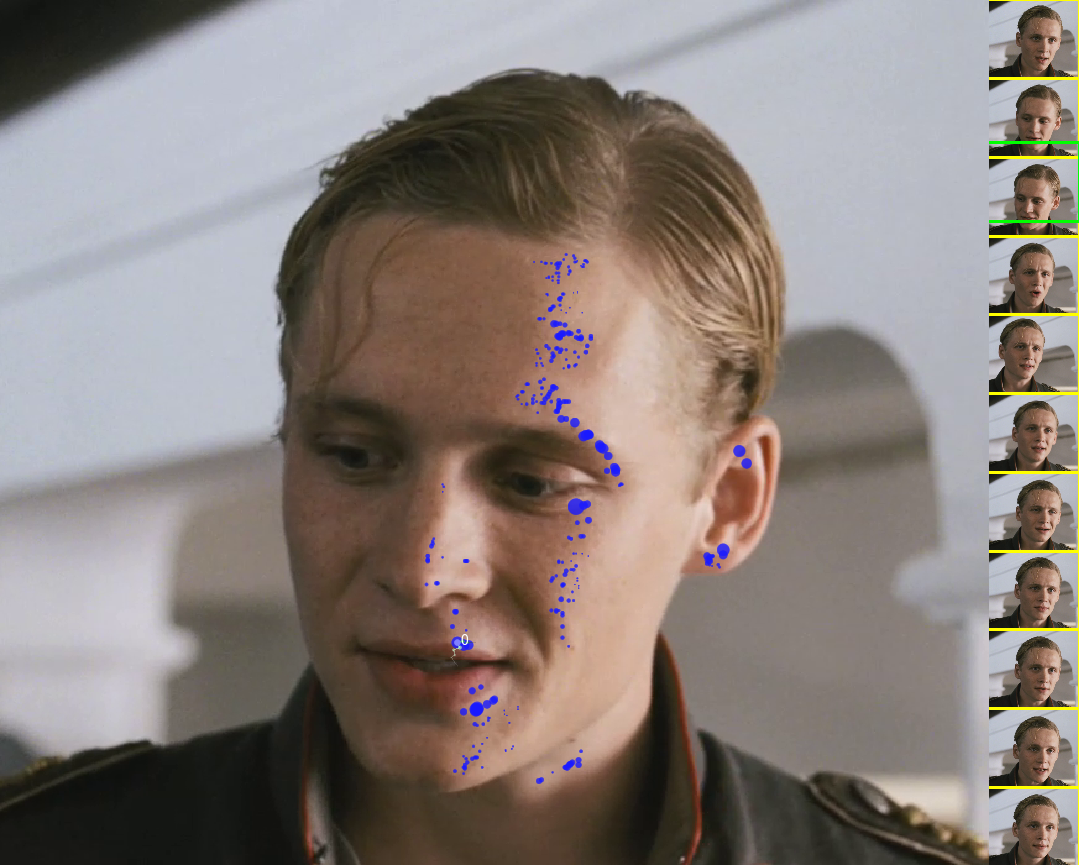
\includegraphics[width=0.46\linewidth]{candidates_lips_ridge_left_bg} &
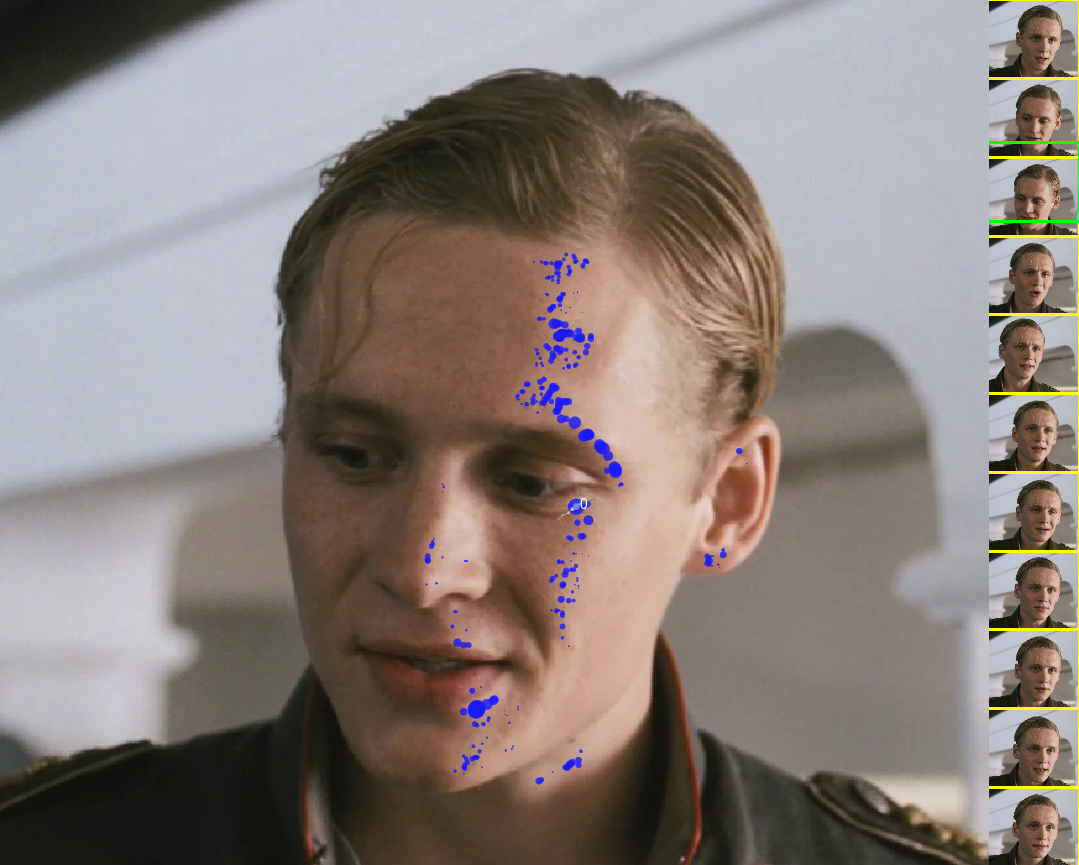
\includegraphics[width=0.46\linewidth]{candidates_lips_ridge_left_no_bg} \\[2em]
%\begin{sideways}{\makebox[0.32\linewidth][c]{Flank of a giraffe}}\end{sideways} & 
%\includegraphics[width=0.40\linewidth]{candidates_giraffes_flank_bg}&
%\includegraphics[width=0.40\linewidth]{candidates_giraffes_flank_no_bg}\\
\end{tabular}
  \indent We incorporate a background model, such that a click tells us not only `this
  is how the landmark looks like', but also `this is how the landmark
  does \emph{not} look like' for all other patches in that frame.

  The figure contrasts the per frame evidence for each candidate patch with and
  without a background model. Using the background model makes the correct
  patch probable enough, that it is chosen. But note that global reasoning over
  the entire path is still necessary, as the correct patch is not the most
  probable patch in this frame.

  The background model is essential for a good user experience, as it avoids
  learning an overly broad apperance model when marking up difficult frames.
   \vspace{0.3em}
  }
%%%%%%%%%%%%%%%%%%%%%%%%%%%%%%%%%%%%%%%%%%%%%%%%%%%%%%%%%%%%%%%%%%%%%%%%%%%%%%
\headerbox{Speed}{name=speed,column=2,row=0,below=results,bottomaligned=background model}{
  %%%%%%%%%%%%%%%%%%%%%%%%%%%%%%%%%%%%%%%%%%%%%%%%%%%%%%%%%%%%%%%%%%%%%%%%%%%%%%
\newcommand{\basiswidth}{0.22}
\newcommand{\basisskip}{0.04} % (1-4*\basiswidth)/3
\newcommand{\imagegrid}[1]{
\begin{tabular}{@{}
  c@{\hspace{\basisskip\linewidth}}%
  c@{\hspace{\basisskip\linewidth}}%
  c@{\hspace{\basisskip\linewidth}}%
  c@{}}
  %
\includegraphics[width=\basiswidth\linewidth,height=\basiswidth\linewidth,keepaspectratio]{#1-01} &
\includegraphics[width=\basiswidth\linewidth,height=\basiswidth\linewidth,keepaspectratio]{#1-02} &
\includegraphics[width=\basiswidth\linewidth,height=\basiswidth\linewidth,keepaspectratio]{#1-03} &
\includegraphics[width=\basiswidth\linewidth,height=\basiswidth\linewidth,keepaspectratio]{#1-04} \\
\includegraphics[width=\basiswidth\linewidth,height=\basiswidth\linewidth,keepaspectratio]{#1-05} &
\includegraphics[width=\basiswidth\linewidth,height=\basiswidth\linewidth,keepaspectratio]{#1-06} &
\includegraphics[width=\basiswidth\linewidth,height=\basiswidth\linewidth,keepaspectratio]{#1-07} &
\includegraphics[width=\basiswidth\linewidth,height=\basiswidth\linewidth,keepaspectratio]{#1-08} \\
\includegraphics[width=\basiswidth\linewidth,height=\basiswidth\linewidth,keepaspectratio]{#1-09} &
\includegraphics[width=\basiswidth\linewidth,height=\basiswidth\linewidth,keepaspectratio]{#1-10} &
\includegraphics[width=\basiswidth\linewidth,height=\basiswidth\linewidth,keepaspectratio]{#1-11} &
\includegraphics[width=\basiswidth\linewidth,height=\basiswidth\linewidth,keepaspectratio]{#1-12} \\
\includegraphics[width=\basiswidth\linewidth,height=\basiswidth\linewidth,keepaspectratio]{#1-13} &
\includegraphics[width=\basiswidth\linewidth,height=\basiswidth\linewidth,keepaspectratio]{#1-14} &
\includegraphics[width=\basiswidth\linewidth,height=\basiswidth\linewidth,keepaspectratio]{#1-15} &
\includegraphics[width=\basiswidth\linewidth,height=\basiswidth\linewidth,keepaspectratio]{#1-16} 
\end{tabular}
}
\noindent\begin{tabular}{@{}c@{\hspace{0.5em}}c@{\hspace{0.5em}}c@{}}
\begin{minipage}{0.3\linewidth}
  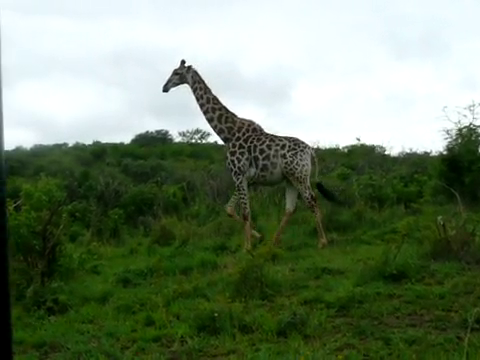
\includegraphics[width=\linewidth]{basis-giraffe-example-frame}\\[1em]
\end{minipage}&
\begin{minipage}{0.3\linewidth}
  \imagegrid{basis-giraffe-basis}
\end{minipage}&
\begin{minipage}{0.3\linewidth}
  \imagegrid{basis-giraffe-response}
\end{minipage}\\
\smaller Image &\smaller  Filter Bank &\smaller  Response
\end{tabular}\\[1em]
\indent{}Speed is achieved by preprocessing the video with an adaptive filter
bank as in~\cite{awf:tracking}. Preprocessing was sped up significantly, but is
still slower than realtime.

This encodes the video into 16 byte per pixel feature vectors. We implemented
an efficient search for similar patches using the SIMD hardware of modern
processors, and only evaluate the cost on these candidate patches. (Typically
200 patches per frame). The Graph-Structure focuses the evaluations on the most
important areas, and makes candidate search and reasoning highly efficient,
such that the system runs at interactive speed.

Note that the preprocessing is not specific to the interestpoints tracked
later. A single preprocessed video can therefore be used in many annotation
sessions.
   \vspace{0.0em}
  }
%%%%%%%%%%%%%%%%%%%%%%%%%%%%%%%%%%%%%%%%%%%%%%%%%%%%%%%%%%%%%%%%%%%%%%%%%%%%%%
  \headerbox{Source Code}{name=source,column=2,below=speed,above=bottom}{
%%%%%%%%%%%%%%%%%%%%%%%%%%%%%%%%%%%%%%%%%%%%%%%%%%%%%%%%%%%%%%%%%%%%%%%%%%%%%%
  \noindent
  \begin{minipage}{\linewidth}
  \begin{minipage}{0.7\linewidth}
    \indent{}The source code and compiled executables with an interactive interface are available at \\
  \end{minipage}\hfill%
  \begin{minipage}{0.28\linewidth}
  \hfill
\includegraphics[width=\linewidth]{chart}
  \end{minipage}
  \end{minipage}
  \url{http://www.cs.unibas.ch/personen/amberg_brian/ Fasttrack}
  }
%%%%%%%%%%%%%%%%%%%%%%%%%%%%%%%%%%%%%%%%%%%%%%%%%%%%%%%%%%%%%%%%%%%%%%%%%%%%%%
  \headerbox{A Future Direction}{name=questions,column=1,span=1,below=background model,above=bottom}{
%%%%%%%%%%%%%%%%%%%%%%%%%%%%%%%%%%%%%%%%%%%%%%%%%%%%%%%%%%%%%%%%%%%%%%%%%%%%%%
    We incorporated a background model, where a click informs us not only that `this is how the
    patch looks like', but also for the rest of the frame, `this is how the patch
    does not look like'. 
    
    Can we also \emph{efficiently} use a background tracks model, allowing us
    to reason, `this would be a good track, but part of it can be better
    explained by tracking another point'.
   \vspace{0.3em}
  }
%%%%%%%%%%%%%%%%%%%%%%%%%%%%%%%%%%%%%%%%%%%%%%%%%%%%%%%%%%%%%%%%%%%%%%%%%%%%%%
  \headerbox{Method}{name=method,column=0,below=contribution,above=references}{
%%%%%%%%%%%%%%%%%%%%%%%%%%%%%%%%%%%%%%%%%%%%%%%%%%%%%%%%%%%%%%%%%%%%%%%%%%%%%%
  \noindent{\centering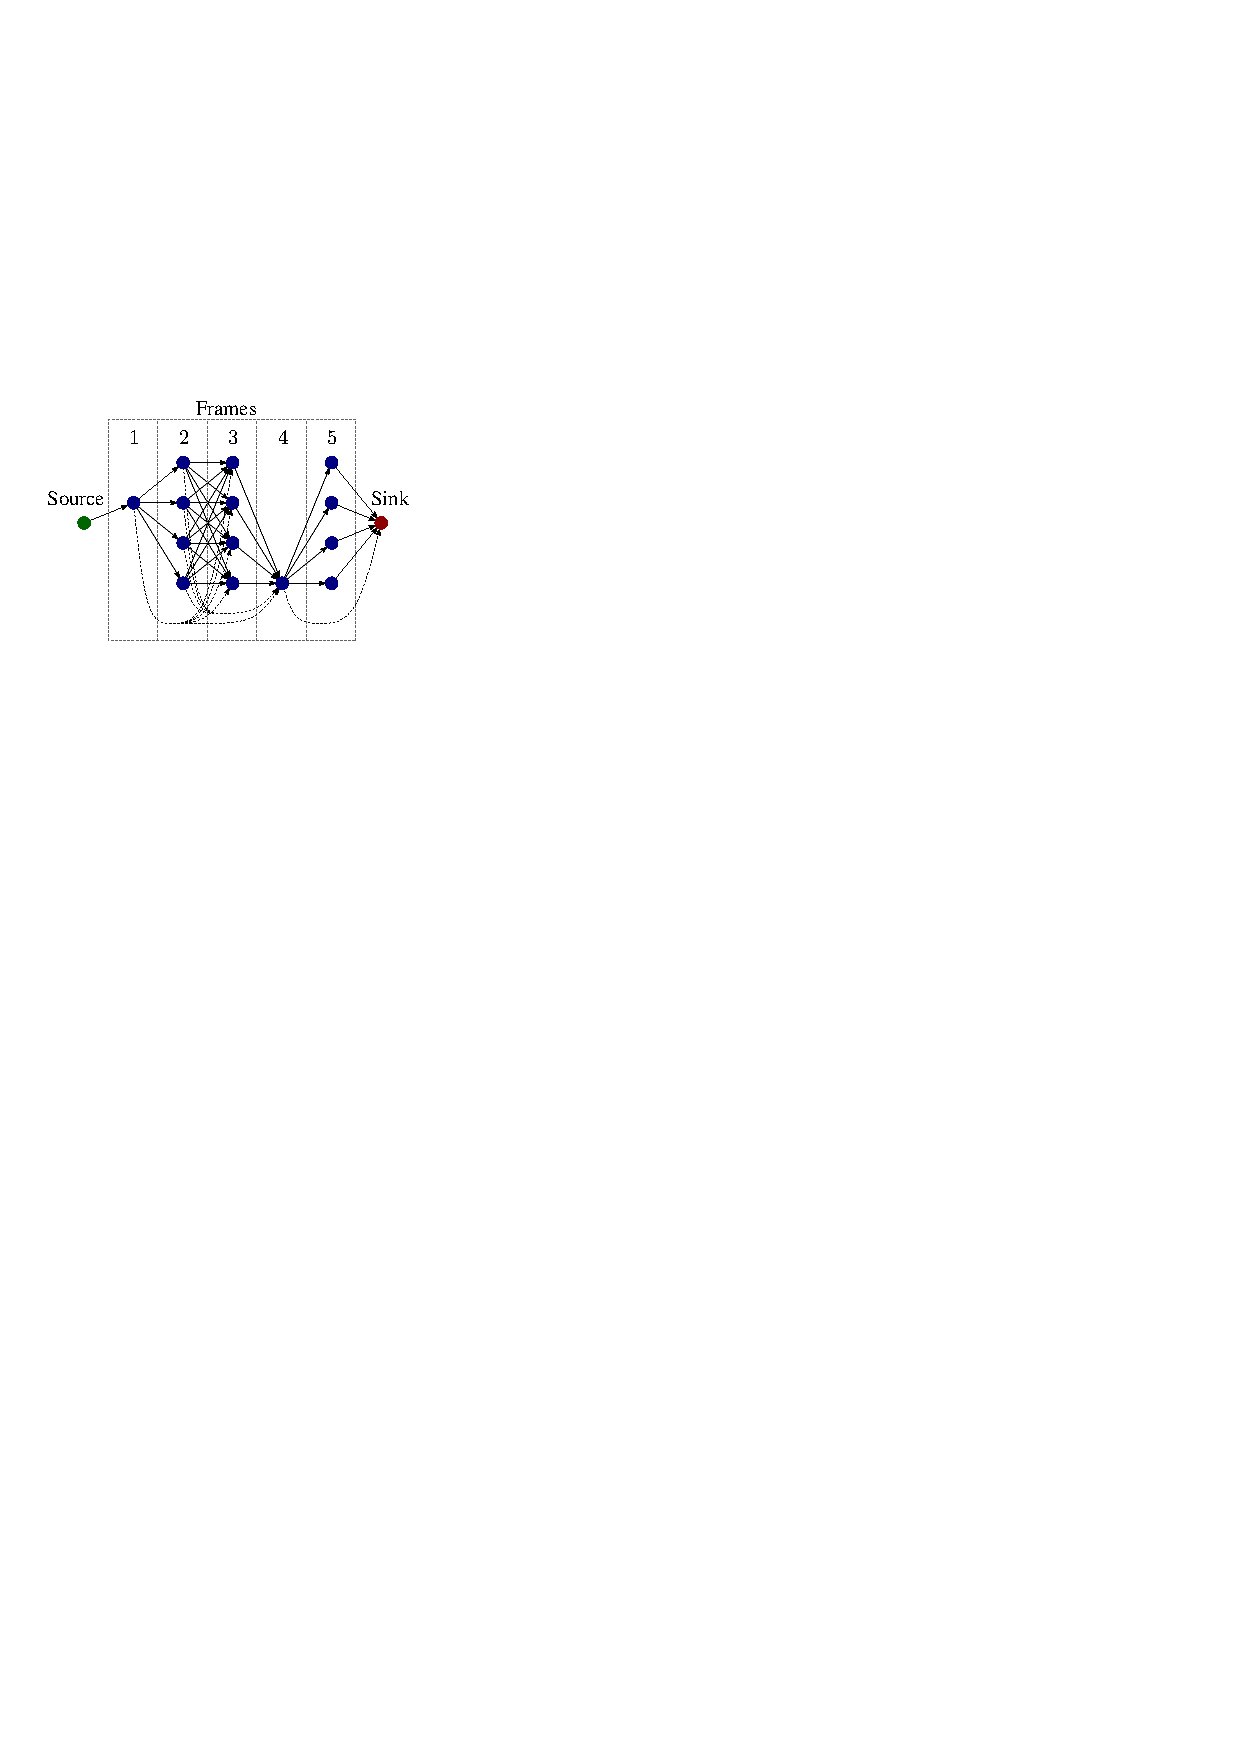
\includegraphics[width=0.95\linewidth]{images/graph_occluded.pdf}\\}
  \indent The cost is interpreted as a directed acyclic graph
  with weights on the nodes and edges. The nodes encode candidate positions,
  and the edges the transition costs between candidates. Additional edges
  (dashed) allow occlusion transitions which skip frames.

  The optimal track is found with a modification of Dijkstra's shortest path
  search. The search was speed up by lower bounding the cost, and lazily
  evaluating the accurate cost only where necessary to find the global optimum.
   \vspace{0.3em}
  }

\end{poster}

\end{document}

